\documentclass[../thesis.tex]{subfiles}

\begin{document}

\chapter{Channel calibration}
\label{chap:calib}

\section{Overview}

For the antineutrino detectors and water pools, the Daya Bay DAQ system outputs little more than timestamped PMT hits, grouped into readout windows and tagged with trigger information. As discussed in \autoref{sec:expADs}, these hits take the form of ADC readings from the peak-finding electronics, along with the TDC count at the time that each (shaped) PMT waveform crossed the disciminator's threshold. In order to carry out any sort of physics analysis, it is necessary to first convert this raw ADC and TDC data into the higher-level quantities of photoelectron count and photon arrival time, and then to combine individual channels into overall event parameters such as energy and position.

This chapter describes the first half of that process; namely, the detector calibration and data processing involved in the channel-by-channel calculation of hit time and charge. (The second half is discussed in \autoref{chap:recon}.) These calibrated quantities are fundamental in that they are used in all further analysis stages and by all reconstruction algorithms. Accuracy is vital, as any bias in the channel charge will be reflected in the total event energy and in any (charge-based) reconstructed vertex; likewise, accurate times are important for time-based vertex reconstructions. Furthermore, it is necessary to identify, exclude, and compensate for any misbehaving channels, a process that will also be discussed here.

\section{Timing calibration}

The timing calibration takes each hit's TDC count\footnote{I.e., the number of ticks that elapsed between the hit and the trigger} and converts it into an estimate of the time at which the photon struck the photocathode. The absolute time is unimportant, but for the purpose of time-based vertex reconstruction (or track reconstruction, as applied in muon studies), the \emph{relative} times between channels must be accurately determined. These calibrated times, in addition to their use in vertex reconstruction, are also used in defining the time window for hit selection (performed during the event-wide charge calculation, described in the next chapter as the first stage of the energy reconstruction).\footnote{Without a hit selection window, the event's total charge could include hits, such as those from dark noise, uncorrelated with the underlying physical event. To be fair, given that this window is 400~ns wide, and any calibration corrections are on the order of a few~ns, the raw times would actually suffice for hit selection.}

This process involves subtracting a channel-specific offset (largely corresponding to cable length) from each channel's hit times, with an additional correction for the charge-dependent \emph{timewalk effect}, in which smaller pulses take longer than larger ones to cross the FEE discriminator's threshold. The offset, as well as a parameterization of the timewalk curve, is stored in the calibration database and applied to the TDC readings during data processing. We now discuss the preparation of these calibration constants.

\subsection{Calibration constant preparation}

To measure each channel's offset and timewalk profile, we require a well-defined event vertex and an external source of $T_0$ (true event time) information.\footnote{There is a natural variance, on the order of 20~ns (XXX check), in the timing of triggers (even for identical calibration events), smearing the TDC measurements between different events. Knowledge of $T_0$ effectively provides knowledge of the trigger ``jitter'' for each event, allowing it to be subtracted out. Without this information, it is difficult to obtain a useful timewalk curve due to the aforementioned smearing.} Toward that end, Daya Bay uses LED calibration runs in which the LED is positioned at the center of the detector. When a pulse is sent to the LED, a ``hit'' is also sent to the FEE from a ``fake'' $T_0$ channel, providing a reference from which other TDCs can be subtracted. For each PMT hit on channel $i$, we take its TDC count $N_i$ and calculate a corrected time
\begin{equation*}
  t_i = \frac{N_0 - N_i}{f_\mathrm{TDC}} - \frac{n r_i}{c},  
\end{equation*}
where $N_0$ is the TDC count of the $T_0$ channel, $f_\mathrm{TDC}$ is the TDC frequency, and $nr_i/c$ gives the time of flight (TOF) to channel $i$, located a distance $r_i$ from the AD's center. The TOF subtraction ensures that we can directly compare channels from different rings without any further geometric considerations. In principle, the resulting $t_i$ should be equal for all channels (modulo the timewalk effects caused by the variation of photon flux for different rings), but in reality, discrete offsets are observed between rings, due to the discretization resulting from the TDC counter's 1.625 (XXX check) period, which is on the same scale as the difference in propagation times between rings. This discretization is not explicitly corrected for, as it does not prevent time-based vertex reconstructions from achieving equal or superior resolution compared to charge-based reconstructions.

In the next step, a 2D histogram is constructed for each channel by taking all of the channel's hits (within a reasonable time window, loosely constructed on the scale of the propagation time between the AD's center and the PMTs) across all events, and plotting each hit's corrected time $t$ against its ADC count $q$. Sampling across $q$ is ensured both by variation of the LED voltage and by the underlying Poisson statistics of photon observation. This histogram's profile is then fit to the six-parameter functional form
\begin{equation*}
  t(q) = a_1 + a_2 \exp (-a_3 q) + a_4 \exp (-a_5 q) + a_6 \log q,
\end{equation*}
which was empirically found to produce good fits under appropriate restrictions on the parameters. \autoref{fig:timewalk} shows an example of a timewalk fit.

After a manual verification of fit quality, the six parameters for each channel were uploaded to the database and marked with a suitable validity period. Whenever the electronics had been modified in a way that could affect the channel timing (for example, a cabling change or a board replacement), a new set of constants was prepared for the affected AD, using this same procedure.

It is worth noting that the $a_1$ parameter can be expressed as $\overline a_1 + \delta a_1$, where $\overline a_1$ is the average value of $a_1$ across all channels, and $\delta a_1$ is the channel-specific deviation. In this case, $\delta a_1$ represents intrinsic (and significant, for such purposes of vertex reconstruction) differences in timing offsets between channels, due to such factors as cable length. Meanwhile, $\overline a_1$ (which arises from, e.g., differences in cable length) has no effect on vertex reconstruction and thus can be removed, meaning that we apply the transformation $a_1 \mapsto a_1 - \overline a_1$. Doing so ensures that, for ordinary physical triggers, the physical hits always fall within the same well-defined band of timewalk-corrected times. If $\overline a_1$ were not removed in this way, then this band would shift as $a_1$ does, which could bias the calculation of the total charge, since this calculation indeed relies on a constant window for hit selection. Removing $\overline a_1$ also ensured that each stored timewalk curve is ``nearly'' zero for large charges (modulo the $a_6$ term), with the deviations from ``nearly'' reflecting the differences in timing offsets between channels.

\begin{figure}[ht]
  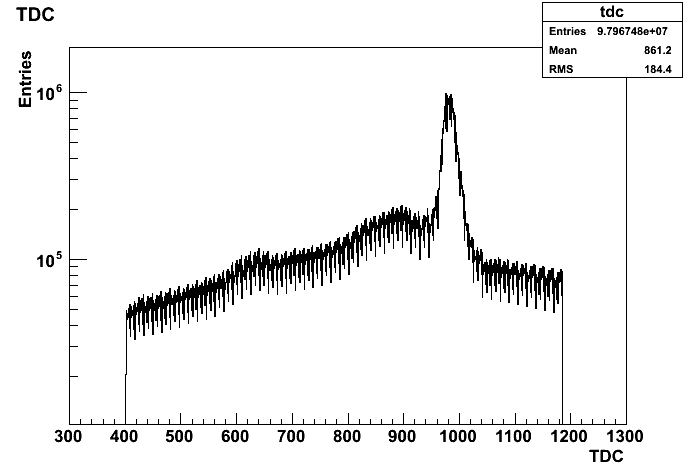
\includegraphics[scale=0.5]{tdc.png}
  \caption{A typical distribution of TDC values for hits in a single PMT during a physics run.}
  \label{fig:tdcDist}
\end{figure}

Due to this last property, the expected time for a ``large'' pulse (for which the timewalk correction is nearly zero), with TDC count $N$, is approximately $-N/f_{mathrm{TDC}}$, where $f_{\mathrm{TDC}} = 1/(1.625\;\text{ns})$. As shown in \autoref{fig:tdcDist}, typical physical hits have TDC counts of 950--1000, corresponding (respectively) to times of -1545 to -1625~ns. The details of selecting physical hits, including the exact range of times used, are discussed in \autoref{sec:reconEnergyCharge}.

% Because $t(q)$ gives the \emph{time since trigger}, which is on the order of a microsecond, a single global $\mu$s-scale offset (the average of all the $a_1$'s, to be precise) is subtracted from each $a_1$. This ensures that when we later use $t(q)$ as a \emph{correction}, we don't apply a large offset to the times we are correcting.

\begin{figure}
  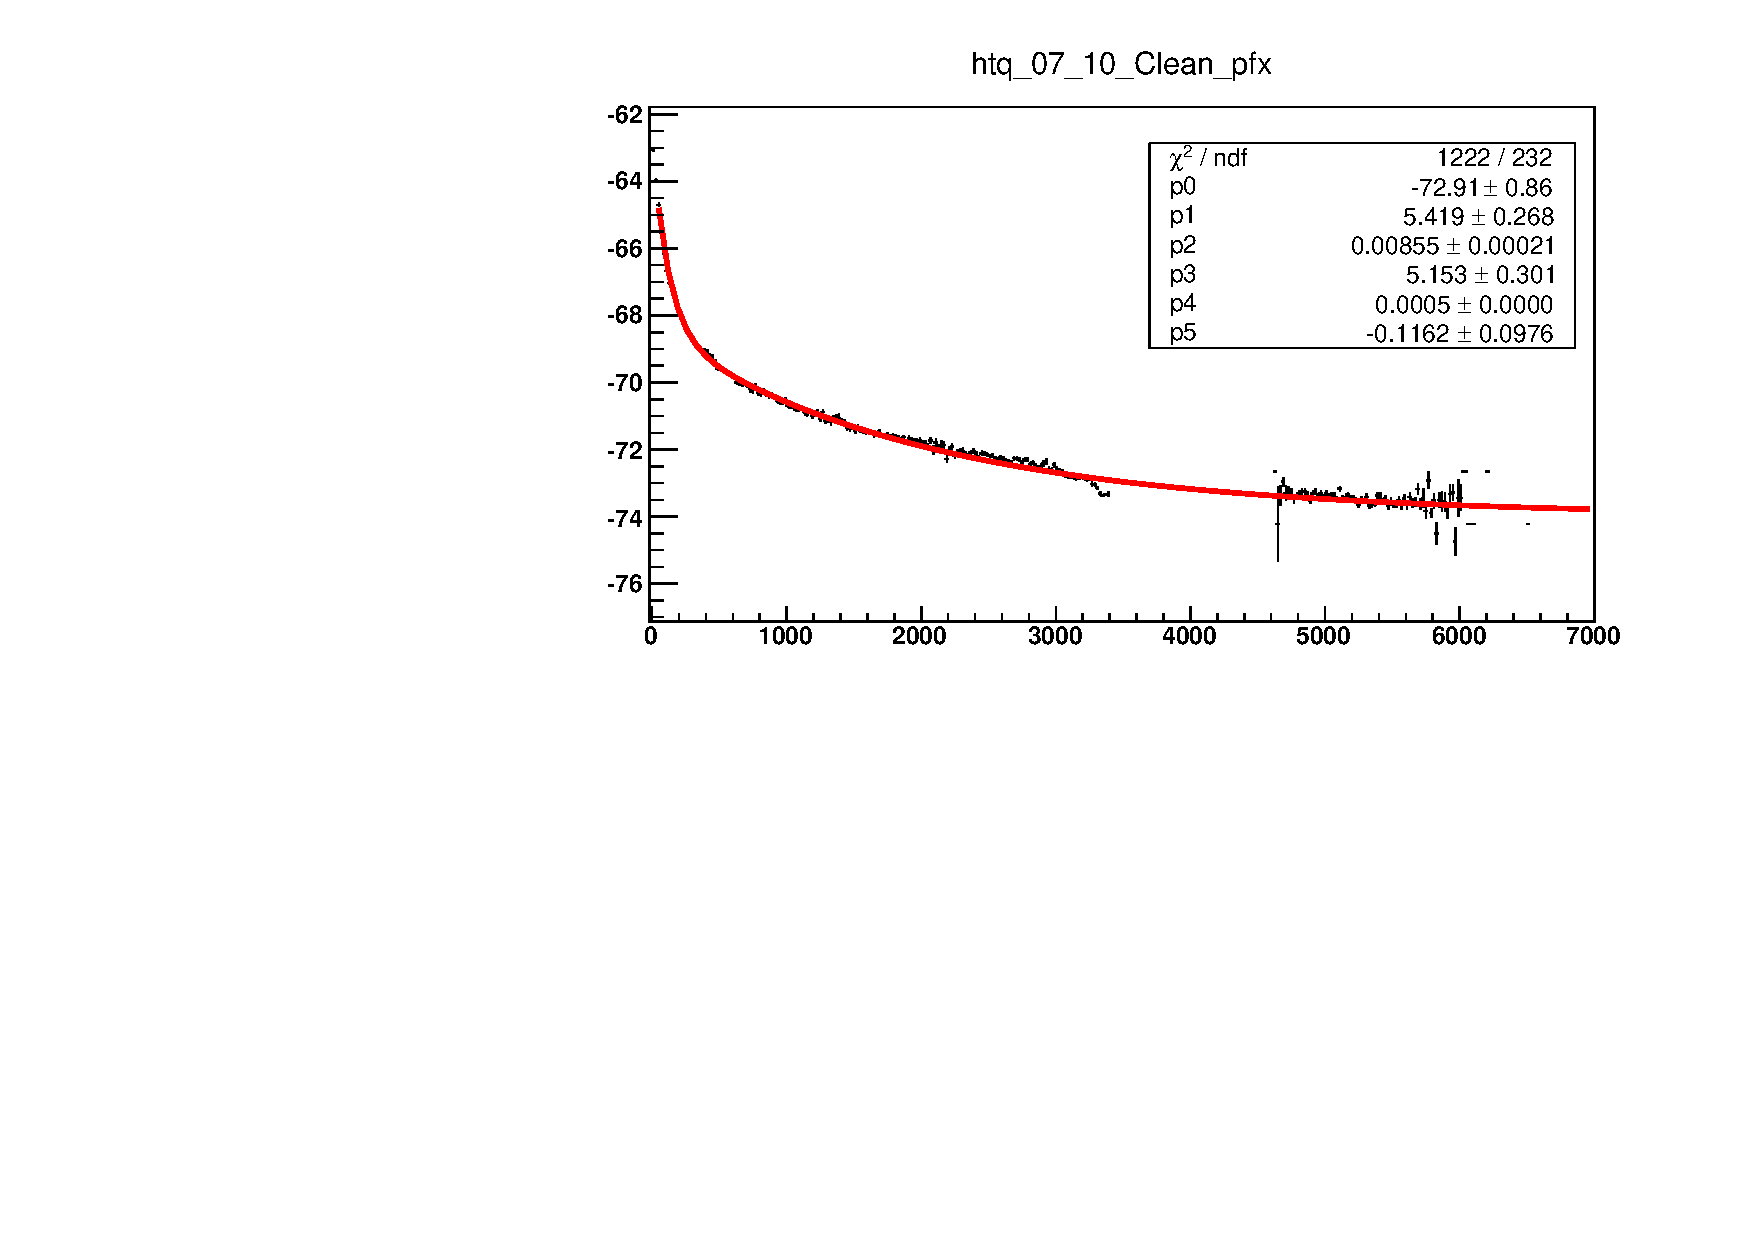
\includegraphics[scale=0.7]{fit_eh1_ad1_r7c10.pdf}
  \caption{An example of a timewalk fit.}
  \label{fig:timewalk}
\end{figure}

\begin{comment}
  Show the tof-corrected times; comment on TDC discretization.
\end{comment}

\subsection{Calculation of corrected times}

Once the calibration parameters are in the database, applying them to the raw data is straightforward. For each hit, we take the ADC count $q$ and plug it into the function $t(q)$, with the parameters taken from the database. Then, using the channel's raw TDC count $N$, the calibrated time $t_c$ is calculated as
\begin{equation}
  \label{eq:corrTime}
  t_c = -\frac{N}{f_\mathrm{TDC}} - t(q),
\end{equation}
After this is done, we have a calibrated time, in nanoseconds (instead of TDC counts), for each hit, which can be directly and accurately compared to other hits in other channels, regardless of how much charge each channel saw and regardless of intrinsic differences between channels. This meets the requirements for time-based vertex and track reconstruction.

\section{Charge calibration}
\label{sec:calibGain}

At a given operating voltage, every PMT will produce a unique amount of charge per photoelectron, even among other PMTs of the same model. Furthermore, the Daya Bay FEE channels have an intrinsic 3\% variation in the number of ADC counts output per unit of charge. As such, the total response of each channel to a single photoelectron, that is, the \emph{total gain}\footnote{Herein, the term \emph{gain} will refer to the total gain (in ADC/PE), and we will use \emph{PMT gain} to refer to the (unitless) gain of the PMT itself.} (in ADC/PE), cannot be precisely predicted based on operating voltage, but instead must be measured \emph{in situ}. Since environmental conditions and the passage of time can alter this response, the gain measurement must be repeated regularly. Once the gain is known, it is possible to determine the total number of photoelectrons observed in an event, regardless (within reason) of any time variation of PMT gains. The gain measurement is described in this section.

Prior to data taking, each PMT underwent benchtop tests in order to estimate an operating voltage that would deliver a PMT gain of $1 \times 10^7 \pm 5\%$. At this gain, the peak voltage of the shaped pulse corresponds to approximately 19 ADC counts, based on the inherent (and fixed) calibration of the ADC. This voltage then remained fixed as long as the gain didn't deviate excessively from the intended range. Minor deviations were acceptable and expected, and were effectively compensated by the gain calibration, provided that the drift occurred over time scales longer than the typical calibration period of $\sim$6 hours. This was indeed the case: Gain drifts were found to occur on a scale of a few percent per year (XXX show plot) 

To measure the gain, Daya Bay uses ``dark noise'', the thermal emission of electrons from the photocathode. Dark noise can be measured ``for free'' during physics data taking by taking advantage of the size of the Daya Bay readout window\footnote{It bears mentioning that in the past, Daya Bay has in fact employed a separate, redundant gain calibration using LED runs, which gave results consistent with this ``rolling gain'' method.}.
\begin{comment}
  \footnote{(WRONG) Each dynode can of course also emit electrons, but the collected charge is attenuated by $\mathcal{O}(5^n)$ for emission from the $n$th dynode. This effect can therefore be safely neglected for our purposes. NOTE: This can't be the reason. A 1/5-scale effect is certainly relevant if dynode thermal emission happens often enough. I believe the actual reason for only considering photocathode emission is that it's the only material that emits electrons at a significant rate (thanks to its work function?).}
\end{comment}
Within a single event, there will be a spread of a few dozen nanoseconds between the hits that correspond to the actual physical event. This timescale is determined by the time it takes light to propagate within the detector volume. Since each readout window is about 1.3~$\mu$s wide, and a trigger is issued about 1~$\mu$s after a physical event takes place, the first few hundred nanoseconds of a readout window serve as an observation of each PMT during detector quiescence\footnote{Dark hits can also be found in the lengthy portion of each readout window following the ``physics'' hits, but since the charge readings can be biased by ringing in the electronics, they are not used in the gain calibration.}. Daya Bay's gain calibration software extracts the hits that lie in this part of each readout, and, after subtracting the ADC pedestal for each hit, constructs a histogram of ADC counts for each channel.

Once the dark noise histogram has accumulated a sufficient number of statistics (six hours' worth) to provide a stable fit, it is fit to a model that includes the total gain as one of the parameters. Thermal emission is modeled as a Poisson process (in terms of the number of photoelectrons), and, in turn, the collected charge per photoelectron is modeled as a Gaussian. Convolving the two then gives the PDF used in the fit:
\begin{equation*}
  P(Q) = \sum_{n^=1}^{\infty} \frac{\mu^n e^{-\mu}}{n!} \frac{1}{\sigma_{\mathrm{SPE}}\sqrt{2n\pi}} \exp\left(-\frac{(Q - n\overline Q^{\mathrm{SPE}})^2}{2n\sigma_{\mathrm{SPE}}^2}\right)
\end{equation*}
where $Q$ is the observed ADC count, $\mu$ (always close to 1) is the mean number of photoelectrons per thermal emission event, $\overline Q^{\mathrm{SPE}}$ is the total gain, and $\sigma_{\mathrm{SPE}}$ is the width of the Gaussian. Due to the extremely low probability of observing multiple thermal electrons in a single hit, the sum was restricted to $n \le 2$ in practice, to negligible effect. This model was found to fit the data stably and precisely as long the fit region was restricted to lie above 10~ADC, below which noise fluctuations had the ability to destabilize the fit.

The results of this fitting procedure were stored in the offline database for use during data production, In cases where a poor fit quality was obtained, a nominal ``default'' value (XXX give number) was stored in the database, making it possible to flag problematic channels by scanning for those that have exactly this value in the database. Similarly, excessively small or large fit gains are used in the determination of channel quality, as discussed in \autoref{sec:calibCQ}.

\subsection{Hit charge calculation}
\label{sec:calibHitCharge}

In the simplest case, the calibrated charge $q$ (in PE) of a hit is related to the raw charge $Q$ (in ADC counts) as
\begin{equation}
  \label{eq:corrChg}
  q = \frac{Q - Q_{\mathrm{pre}}}{\overline Q_{\mathrm{SPE}}}.
\end{equation}
Here, $Q_{\mathrm{pre}}$ is the pre-ADC value described in \autoref{sec:expPmtElec} (i.e. the average of the four ADC samples preceding the over-threshold instant of the discriminator), and $\overline Q^{\mathrm{SPE}}$ is the calibration constant retrieved from the offline database for the particular PMT and time period in question. This calculation is fairly reliable as long as a hit is not preceded by any other hits within $\sim$300~ns.

When hits are more closely spaced in time, however, the calculation is made more complicated by the peculiar behavior of the electronics, as illustrated in \autoref{fig:closeHitsExamples}. This peculiarity can be boiled down to two facts. First of all, the peak-finding algorithm always takes the largest sample within a continuous series of above-baseline samples, even when this causes the same peak to be reported for more than one hit (see the first three columns of \autoref{fig:closeHitsExamples}). And secondly, the pre-ADC of a hit can be biased by the preceding hit (see the last two columns of \autoref{fig:closeHitsExamples}). 

\begin{figure}[ht]
  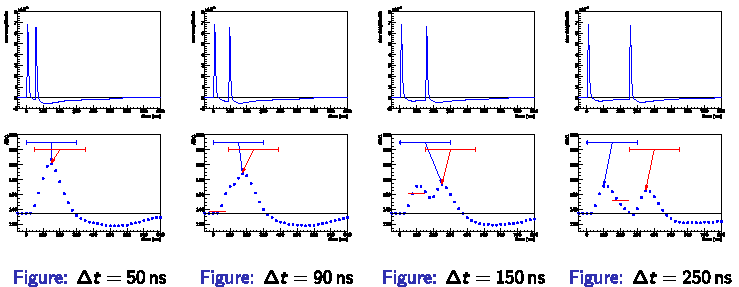
\includegraphics[scale=1.2]{closeHitsExamples.pdf}
  \caption{An illustration of the different scenarios that can occur when dealing with closely spaced hits. In this case, each hit is one photoelectron. The red dashed lines are the pre-ADC values \emph{for the second hit}. From XXX doc-6710}
  \label{fig:closeHitsExamples}
\end{figure}

Simply using \eqref{eq:corrChg} for all hits will result in over or underestimating the total charge, depending on the time separation between hits, as illustrated by the green/gray dots in \autoref{fig:closeHits}. For separations of less than $\sim$100~ns, the peak finder will approximately report the correct \emph{total} charge, but this charge will be assigned to two hits and will thus be double counted. This is shown in the first two columns of \autoref{fig:closeHitsExamples}. For separations of $\sim$100--250~ns, the samples will not reach baseline and thus a single peak value will still be reported twice, but in this case the peak's amplitude is low enough that double-counting it will more closely approximate the total charge than single-counting it. However, the pre-ADC for the second hit is biased by the samples from the first hit, and so this pre-ADC should be discarded in favor of the one from the first hit. Finally, for separations greater than $\sim$250~ns, the samples will hit the baseline in between the peaks, so two different peak values will be reported, and both should be used, but once again, the pre-ADC for the second hit may be biased by the first hit (whose shaped pulse includes an undershoot that extends for several hundred ns beyond the positive pulse).

On account of this behavior, an algorithm was designed (XXX doc 6710) with the goal of minimizing the overall bias in the total charge (as studied under the scenario of two SPE hits). In what follows, $\Delta t$ is the time since the previous hit in the same readout:

\begin{enumerate}
\item If the hit is the first one in the readout, treat it simply using \eqref{eq:corrChg}.
\item If $\Delta t < \SI{100}{ns}$, set the hit's calibrated charge to zero. In this case the aim is to avoid double-counting the total charge, as illustrated in the first two columns of \autoref{fig:closeHitsExamples}.
\item If $\Delta t \ge \SI{100}{ns}$, and the peak value is the same as that of the previous hit, use the pre-ADC of the \emph{previous} hit. This avoids the bias on the second pre-ADC value, as shown in the third column of \autoref{fig:closeHitsExamples}.
\item If $\Delta t \ge \SI{100}{ns}$ and a \emph{different} peak values is reported, ignore the hit's pre-ADC, and instead subtract the parameterized tail shape of the previous pulse (as this tail is essentially the ``true'' pedestal of the hit). This method, dubbed \emph{charge correction}, was developed by the author.
\end{enumerate}

However, studies showed that the overall effect (on resolution and bias of reconstructed energy) of the undershoot correction was negligible, at the cost of considerable operational complexity (in maintaining the parameterization of the pulse shapes). In the end, the algorithm as implemented goes:

\begin{enumerate}
\item If the hit is the first one in the readout, again treat it simply using \eqref{eq:corrChg}.
\item If $\Delta t < \SI{100}{ns}$, \emph{and the peak value is the same as that of the previous hit}, set the hit's calibrated charge to zero.
\item If $\Delta t \ge \SI{100}{ns}$, \emph{whether the peak value is the same as or diffrent from the previous one}, use the pre-ADC from the \emph{previous} hit.
\item \emph{(Special case)} If $\Delta t < \SI{100}{ns}$, and the peak value is \emph{different}, treat the hit simply using \eqref{eq:corrChg}. The reasoning for this special case does not seem to be documented, and it likely only applies to the (rare) scenario of two closely spaced sub-SPE hits, for which it may be possible for the ADC to hit baseline in between the two peaks. In this scenario, keeping both hits may produce a more accurate charge measurement.
\end{enumerate}

\begin{figure}[ht]
  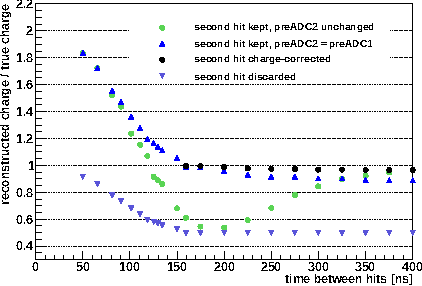
\includegraphics[scale=1.6]{closeHits.pdf}
  \caption{Biases induced by different methods of handling closely spaced hits. Modified from XXX doc-6710.}
  \label{fig:closeHits}
\end{figure}

This algorithm is illustrated in \autoref{fig:closeHits}, which shows how this ``piecewise'' calculation reduces the overall bias compared to the naive application of \eqref{eq:corrChg} to all hits. In practice, however, only the \emph{first} hit (within a specified time window) is used in reconstructing the energy of an event. The reasons for this, and the details of the reconstruction, are discussed in \autoref{sec:reconEnergyCharge}.

\subsubsection{Single-channel electronics nonlinearity correction}
\label{sec:calibSCNL}

XXX to be continued.

\section{Channel quality}
\label{sec:calibCQ}

In order to prevent any biases from being introduced by problematic channels, a channel quality database is consulted during data production, and any tagged channels are excluded from the total event charge (see \autoref{sec:reconEnergyCharge}). Bad channels are identified and tagged during the regular ``keep-up'' processing of each new data file. Four criteria are used for each channel. For ordinary physics runs\footnote{Given that calibration runs feature a different population of events compared to physics runs, these runs use alternative acceptible ranges of occupancy and ADC, determined by observation. In all other respects, channel quality determination is the same for these runs.}, these conditions are as follows (evaluated once for each data file, corresponding to $\sim$10 (30) minutes of DAQ time in a near (far) hall AD):

\begin{enumerate}
\item The occupancy (i.e., the percentage of events in which the channel recorded at least one hit) must be between 0.1 and 0.65/0.5 (near/far). Too low of an occupancy would imply a dead or dying channel, and too high would indicate a noisy channel.
\item The high voltage must be at least 1200~V. A low HV would indicate a problem with the HV supply, requiring the exclusion of the channel from the charge sum.
\item The RMS variation of the HV, during the time span of the data file, must be less than 0.5 V. Anything higher would indicate an unstable HV supply and hence an unstable gain.
\item The baseline-subtracted ADC count, on average, must be between 10 and 45~ADC. This range is based on observations, and its relatively large spread is due to the differences in the average amount of light seen by PMTs near the top and bottom, relative to those near the center.
\end{enumerate}

These four ``ingredients'', as well as the ``good or bad'' verdict, are stored in a dedicated channel quality (CQ) database during keep-up production. In turn, an automated batch job takes the verdicts, compresses them into bitfields, and inserts them into the main offline database, from which they are taken during event charge calculation. If, at a later date, a decision is made to revise the cuts used in the channel quality determination, the ``ingredients'' can be taken from the CQ DB and a new verdict can be made, without any need to revisit the underlying data file. In practice, however, the Daya Bay CQ cuts have proven to be robust enough not to require revision (XXX check).

\subfilebackmatter
\end{document}
